% !TeX spellcheck = de_CH
%%%%%%%%%%%%%%%%%%%%%%%%%%%%%%%%%%%%%%%%%%%%%%%%%%%%%%%%%%%%%%%%%
%  _____   ____  _____                                          %
% |_   _| /  __||  __ \    Institute of Computitional Physics   %
%   | |  |  /   | |__) |   Zuercher Hochschule Winterthur       %
%   | |  | (    |  ___/    (University of Applied Sciences)     %
%  _| |_ |  \__ | |        8401 Winterthur, Switzerland         %
% |_____| \____||_|                                             %
%%%%%%%%%%%%%%%%%%%%%%%%%%%%%%%%%%%%%%%%%%%%%%%%%%%%%%%%%%%%%%%%%
%
% Project     : BA Welti Keller
% Title       : 
% File        : hardware.tex Rev. 00
% Date        : 15.09.2014
% Author      : Tobias Welti
%
%%%%%%%%%%%%%%%%%%%%%%%%%%%%%%%%%%%%%%%%%%%%%%%%%%%%%%%%%%%%%%%%%

\chapter{Hardware-Konzept}\label{chap.hardware}

\todo{Hardware}

\section{Hardware-Architektur}\label{sec.hw_arch}

Anhand der funktionalen Vorgaben für die Messstation werden der \gls{logger}, die \gls{sensoreinh} und das Bussytem im folgenden genauer spezifiziert und die Komponenten ausgewählt.

\subsection{Datenlogger}
Das \gls{hardware}-Konzept des \gls{logger}s ist in Abbildung \ref{fig.hwkonzept_logger} dargestellt.
Der \gls{logger} sammelt die Daten der \glspl{sensoreinh} über das \gls{bussys} ein und speichert sie ab. Dafür benötigt er das \gls{bussys}, einen \gls{mc}, internen Speicher und ein leicht auswechselbares \gls{speichermedium}. Ausserdem soll über eine Schnittstelle ein Computer angeschlossen werden können, um den Betrieb der Messstation zu steuern. Der \gls{logger} wird in einem wasserdichten Gehäuse untergebracht. Für den Austausch des \gls{speichermedium}s wäre eine verschraubbare Öffnung denkbar.

\begin{figure}
	\centering
		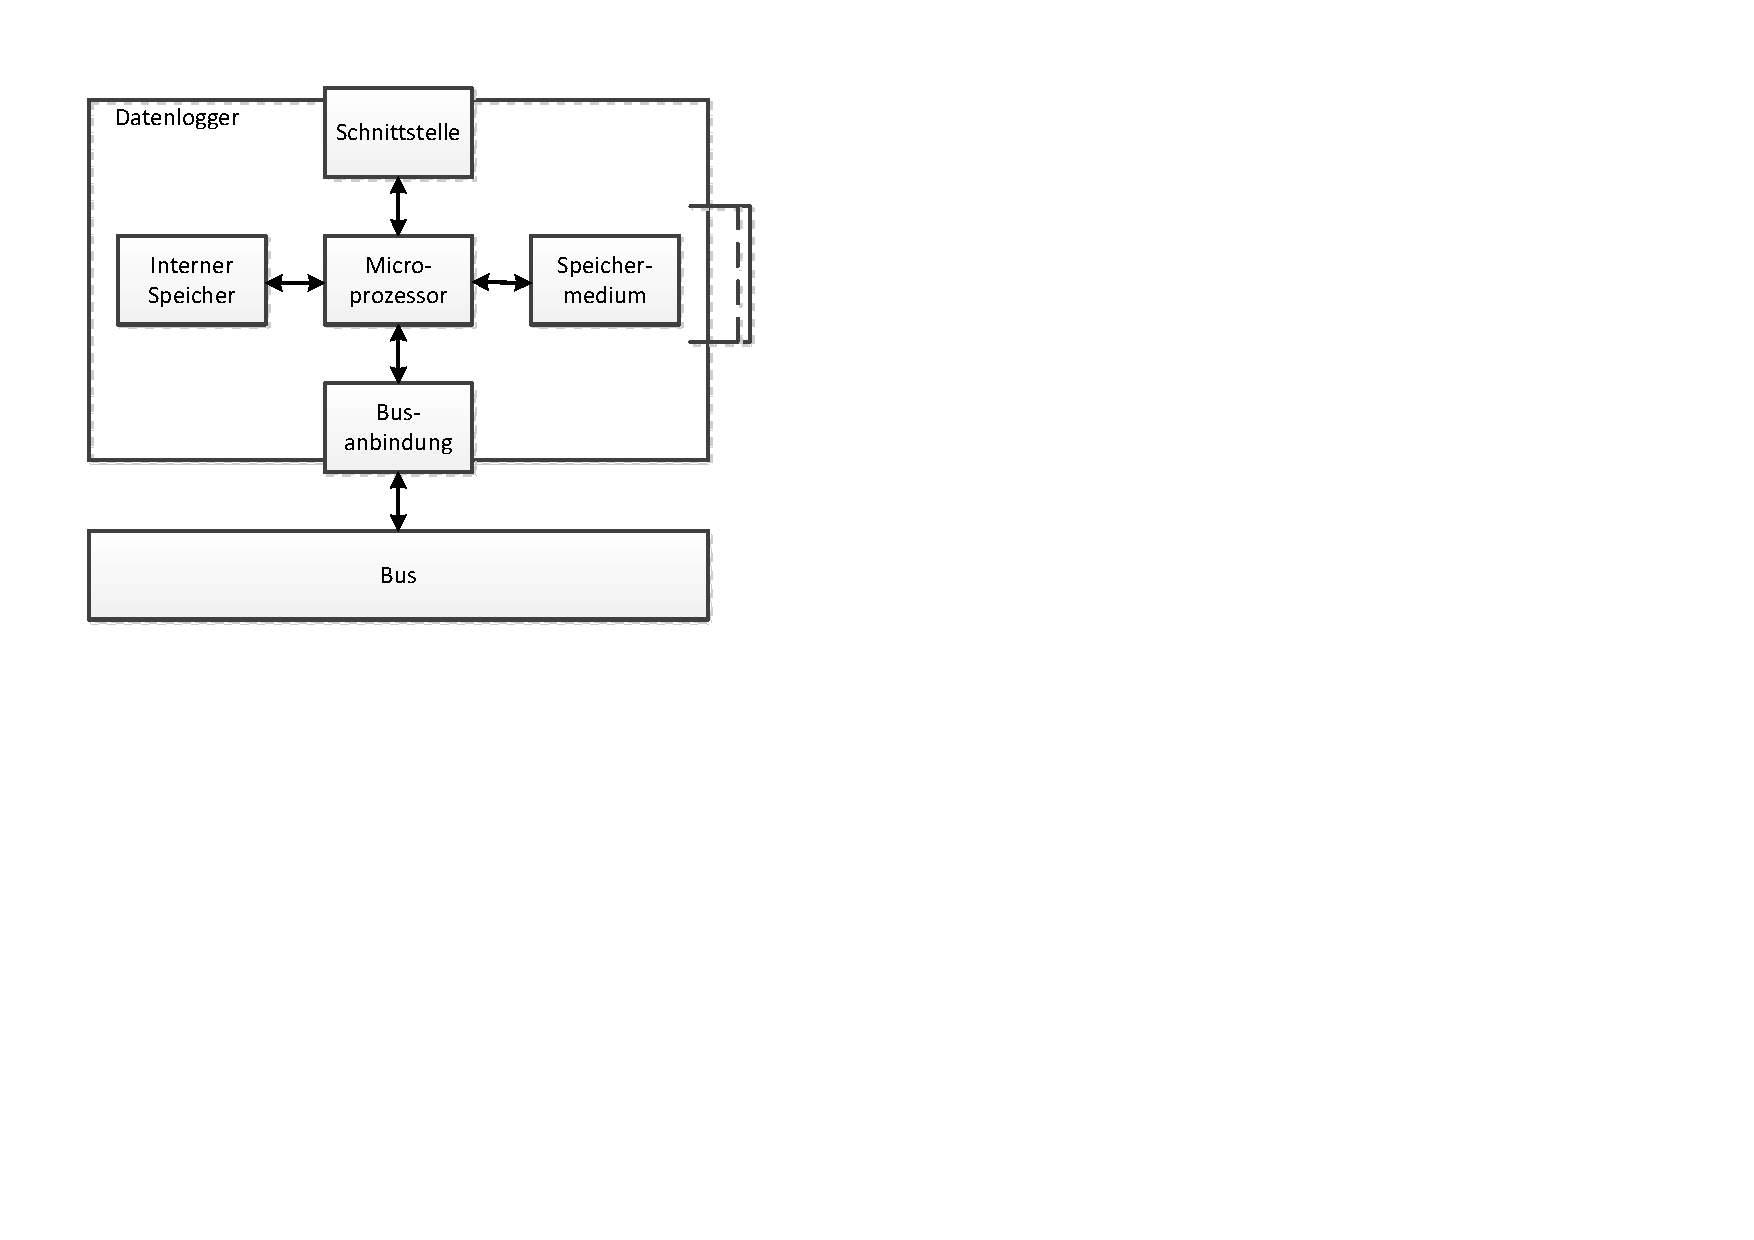
\includegraphics[width=0.8\textwidth]{images/visio/hardwarekonzept_logger.pdf}
	\caption{Hardwarekonzept des \gls{logger}s.}
	\label{fig.hwkonzept_logger}
\end{figure}

\subsection{Sensoreinheit}
Die \gls{sensoreinh} benötigt einen Beschleunigungssensor, um die Einschläge von Geschiebe zu messen. Über einen Analog-Digital-Wandler (\gls{adwandler}, Englisch \gls{adc}) werden die Messsignale digitalisiert. Die gemessenen Signale werden von einem \gls{mc} verarbeitet, im internen Speicher zwischengespeichert und über das \gls{bussys} an den \gls{logger} übertragen. Abbildung \ref{fig.hwkonzept_sensor} zeigt das \gls{hardware}-Konzept der \gls{sensoreinh}.

\begin{figure}
	\centering
		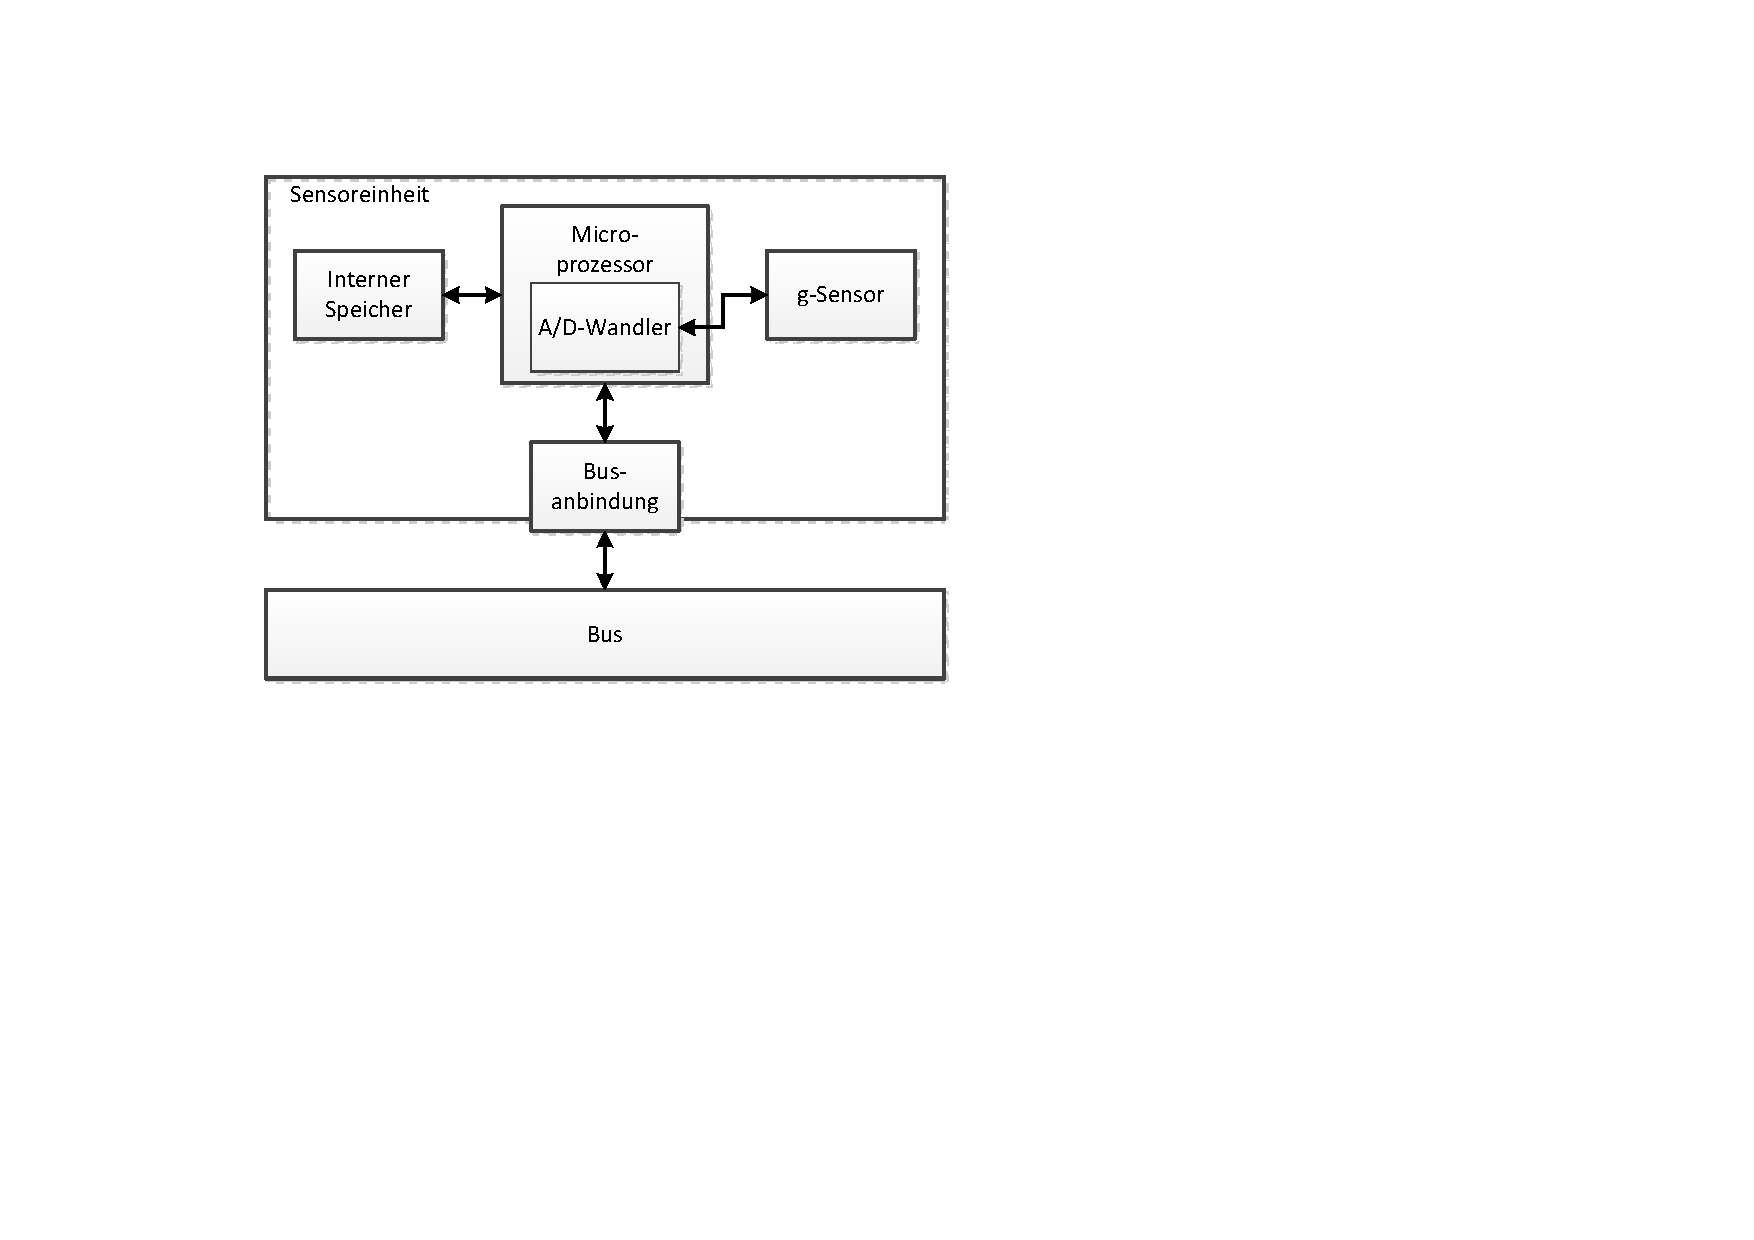
\includegraphics[width=0.8\textwidth]{images/visio/hardwarekonzept_sensor.pdf}
	\caption{Hardwarekonzept der \gls{sensoreinh}.}
	\label{fig.hwkonzept_sensor}
\end{figure}

\subsection{Bussystem}
Das \gls{bussys} muss die Daten und Befehle zwischen \gls{logger} und \glspl{sensoreinh} übertragen. Die Reichweite des \gls{bussys}s muss genügen, um alle Komponenten der Messinstallation zu verbinden. Die Datenbandbreite muss die Übertragung der Messresultate aller \glspl{sensor} erlauben.


\section{Komponentenauswahl}

\subsection{Mikroprozessor}
Bei der Auswahl des \gls{mc}s werden folgende Kriterien berücksichtigt:

\begin{itemize}
\item Genügend Rechenleistung für allfällige zusätzliche Anforderungen.
\item \gls{adwandler} mit genügender Abtastrate und Auflösung (\gls{bitbreite}).
\item \gls{dspgloss} integriert für die schnelle Verarbeitung der Messdaten.
\item \gls{nvic}.
\item Ein-/Ausgänge für das \gls{bussys}.
\item Ein-/Ausgänge für den externen Speicher.
\item möglichst geringer Stromverbrauch.
\end{itemize}

Für die vorliegende Anwendung eignen sich Mobile-Prozessoren sehr gut. Sie sind für den Einsatz in mobilen Geräten konzipiert, d.h. für den Batteriebetrieb, sind aber trotzdem sehr leistungsfähig. Die \emph{ARM Cortex}-Reihe bietet ein breites Spektrum an Prozessoren an. Im Mobile-Segment der \emph{ARM Cortex}-Reihe sind vier Prozessoren erhältlich. Da nur ein Modell einen \gls{dsp} aufweist, ist die Entscheidung einfach. Der \emph{ARM Cortex-M4} ist auch der neueste Prozessor aus dem Mobile-Segment. Mit dem Ausblick, das Messsystem in einem zukünftigen Projekt zur Serienreife zu bringen, macht es nur Sinn, den neuesten Prozessor zu verwenden. Ein Auszug aus dem Datenblatt des \emph{ARM Cortex-M4} befindet sich im Anhang \ref{ds.lpc4088}. Abbildung \ref{fig.M4diagramm} zeigt die Fähigkeiten des \emph{ARM Cortex-M4}.

\paragraph{\gls{nvicgloss}} Ein Prozessor mit NVIC kann auf verschiedene Ereignisse reagieren, indem Interrupts ausgelöst werden. Jedem Interrupt kann eine Priorität zugewiesen werden, um festzulegen, ob ein Interrupt einen anderen unterbrechen darf, der gerade vom Prozessor abgearbeitet wird. Für das Messsystem wird ein \gls{nvic} benötigt, da mehrere zeitkritische Prozesse parallel ablaufen sollen. Einerseits muss die Abtastrate der Messwerterfassung genau eingehalten werden. Andererseits darf die Verarbeitung der Messwerte nicht zu lange unterbrochen werden, um einen Überlauf der Queue zu vermeiden. Die Daten der \glspl{ereignis} müssen parallel dazu an den \gls{logger} übermittelt werden. Die Prioritäten dieser Prozesse müssen richtig gewählt werden. Im Abschnitt \ref{sec.parallel} wird näher darauf eingegangen.

\paragraph{\gls{dsp}} Der \emph{ARM Cortex-M4} verfügt über \gls{dsp}-Funktionen, eine sog. single-cycle \gls{mac}. In einer single-cycle \gls{macgloss} können Multiplikationen in einem einzigen Prozessorzyklus ausgeführt werden. Normalerweise benötigt ein Prozessor für eine Multiplikation bis zu mehreren zehn Zyklen, bis das Resultat vorliegt. Mit einem \gls{dspgloss} ist es daher möglich, z.B. eine Filterfunktion viel effizienter zu berechnen als mit einem normalen Prozessor, da für diese viele Multiplikationen und Additionen ausgeführt werden müssen.

\paragraph{\gls{fpu}} Eine \gls{fpugloss} führt Berechnungen mit Dezimalbrüchen sehr rasch aus. Für unsere Anwendung ist eine \gls{fpu} keine Voraussetzung. Falls in einem späteren Projekt komplexere Filter oder andere Anwendungen berechnet werden müssen, könnte die \gls{fpu} aber ein Vorteil sein.

\paragraph{Wake Up Interrupt Controller Interface} Ein Wake Up Interrupt Controller Interface ermöglicht es, einen Prozessor in einen Stromsparmodus zu versetzen und ihn durch ein definiertes Signal wieder zu wecken. Damit ist es möglich, eine \gls{sensoreinh} praktisch ganz abzuschalten, wenn sie keine Messungen durchführt. Durch eine Nachricht über das Bussystem kann die \gls{sensoreinh} wieder eingeschaltet werden. Der Cortex-M4 verfügt über 240 mögliche Wake Up Interrupts, kann also für 240 Ereignisse programmiert werden, die ihn aufwecken oder in einen Stromsparmodus senden können (vgl. \cite{armcortex}).

\begin{figure}
	\centering
		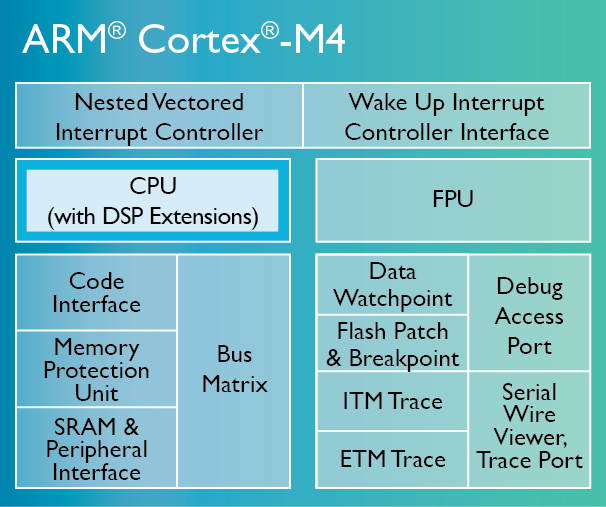
\includegraphics[width=0.8\textwidth]{images/datasheets/Cortex-M4-chip-diagram-LG.png}
	\caption{Chipdiagramm der \emph{ARM Cortex-M4} Architektur \cite{armcortex}.}
	\label{fig.M4diagramm}
\end{figure}

\paragraph{Rechenleistung} Die Rechenleistung des \emph{ARM Cortex-M4} hängt von der Implementation ab. Die Firma ARM produziert den \emph{ARM Cortex-M4} nicht selbst, sondern lizenziert Chip-Hersteller für die Verwendung der Architektur in ihren Prozessoren. Vom \emph{ARM Coretx-M4} sind mehrere Ausführungen erhältlich. Verschiedene Chip-Hersteller implementieren eine Architektur des \emph{ARM Cortex-M4} in ihren Prozessoren.

\paragraph{\gls{adwandler}} Bei den bestehenden Messstationen wird die Datenmenge stark reduziert, indem über eine Minute ein Histogramm mit den Peakintensitäten als Klassen berechnet wird. Die Intensitäten werden in 18 Klassen logarithmischer Abstufung eingeteilt. Das entspricht einer \gls{bitbreite} von etwas mehr als vier Bit (4 Bit ermöglichen 16 Werte). Da für die Klasseneinteilung eine logarithmische Abstufung gewählt wurde, muss ein linearer \gls{adwandler} trotzdem eine höhere \gls{bitbreite} als vier aufweisen, um die gleiche Auflösung wie in den unteren logarithmischen Klassen zu erreichen. Mit 12 Bit Auflösung sind 4096 Stufen unterscheidbar, was für diese Anwendung genügt.

\paragraph{Peripherie} Damit der Prozessor über das Bussystem kommunizieren und auf ein externes Speichermedium schreiben kann, sind genügend Ein- und Ausgabe-\glspl{pin} nötig.

\paragraph{Wahl eines Prozessors} Da der Entscheid für eine Hardware schon zu Beginn des Projekts gefällt werden musste, wurde auf eine grosszügige Sicherheitsmarge in Sachen Rechenleistung und \gls{bitbreite} geachtet.  Um Kosten und Baugrösse der \gls{sensoreinh} klein zu halten, suchten wir nach einem Evaluationsboard mit \emph{ARM Cortex-M4} Prozessor. Das \emph{LPC4088 QuickStart Board} von \emph{NXP Semiconductors} hat genügend Arbeitsspeicher für den Prozessor, verfügt über die benötigten \glspl{pin} für die Peripherie und hat bei weitem genügend Rechenleistung. Die Fähigkeiten des NXP LPC4088FET208 Prozessors sind in Tabelle \ref{table.lpc4088} dargestellt. 

\begin{table}
\begin{center}
\begin{tabular}{|l|l|}
\hline
Taktfrequenz & bis 120 MHz \\
\hline
NVIC & vorhanden \\
\hline
FPU & vorhanden \\
\hline
Programmspeicher & 512 kByte \\
\hline
Arbeitsspeicher (intern) & 96 kByte \\
\hline
CAN-Bus & 2 \\
\hline
USB & 2 \\
\hline
SD-Card & Anschlüsse vorhanden \\
\hline
\gls{adwandler} & 8 Eingänge, 12 Bit \\
\hline
\end{tabular}
\caption{Fähigkeiten des NXP LPC4088 Prozessors \cite{nxplpc4088}.}
\label{table.lpc4088}
\end{center}
\end{table}

Auf dem \emph{NXP LPC4088 QuickStart Board} sind zusätzliche Bauteile verbaut, z.B. Speicher (\gls{sdram} und \gls{flash} und \gls{pin}-Steckleisten, um CAN-Bus-\glspl{pin} oder A/D-Eingänge anzuschliessen. Tabelle \ref{table.nxplpc4088qsb} listet die für dieses Projekt relevanten, zusätzlichen Eigenschaften auf.

\begin{table}
\begin{center}
\begin{tabular}{|l|l|}
\hline
Prozessor & NXP LPC4088FET208\\
\hline
Taktfrequenz & bis 120 MHz \\
\hline
Flash-Speicher & 8 MByte \\
\hline
SDRAM & 32 MByte \\
\hline
\gls{adwandler} & 6 Eingänge nutzbar, 12 Bit \\
\hline
\end{tabular}
\caption{Zusätzliche Fähigkeiten des NXP LPC4088 QuickStart Boards von \emph{Embedded Artists}  \cite{nxplpc4088qsb}.}
\label{table.nxplpc4088qsb}
\end{center}
\end{table}

\subsection{Bus-System}
Das \gls{bussys} für die Messanlage muss die folgenden Kriterien erfüllen:
\begin{itemize}
\item Übertragungsbandbreite genügend für fortlaufende Übertragung von Rohdaten einer \gls{sensoreinh}.
\item Reichweite mindestens 20 Meter.
\item Robust gegenüber äusseren Einflüssen.
\item Mindestens zwanzig Busteilnehmer möglich.
\end{itemize}

\begin{table}
\begin{tabular}{|l|l|l|l|l|}
\hline  & \textbf{Bitrate}      & \textbf{Distanz} & \textbf{Clients} & \textbf{Besonderheiten}\\ 
\hline \textbf{CAN} & \begin{minipage}{2cm}
1 MBit/s\\ 125 kBit/s
\end{minipage} & \begin{minipage}{1.5cm}40 m\\500 m\end{minipage} & > 20 & \begin{minipage}{6cm}
\mbox{ }\\+ \gls{cdet} umgehen mit \gls{polling} durch Master.\\
+ Bei synchronem CAN wird \gls{cdet} durch ID gelöst.\\
+ CAN Controller sendet Interrupt Request bei erhaltener Nachricht.\\
\end{minipage} \\ 
\hline \textbf{SPI} & ..100 MBit/s & < 1 m & \begin{minipage}{1cm}
slave select
\end{minipage} & \begin{minipage}{6cm}
\mbox{ }\\- Pro Client eine Slave Select Leitung\\
- alternativ: \gls{daisy} $\Rightarrow $alle \gls{mcacr} beschäftigt.\\
- Bei Ausfall eines \gls{mcacr} ganzer Bus unterbrochen.\\
\end{minipage} \\ 
\hline \textbf{RS485} & \begin{minipage}{2cm}
35 MBit/s\\100 kBit/s
\end{minipage} & \begin{minipage}{1.5cm}
10 m\\1200 m
\end{minipage} & >32 & \begin{minipage}{6cm}
\mbox{ }\\- Master am besten in der Mitte des Bus $\Rightarrow$ ungünstig.\\
- Braucht 2..4 Drähte (bei Full Duplex)\\
- braucht pull-up und pull-down Widerstände $\Rightarrow$ mehr Leistungsaufnahme.\\
\end{minipage} \\ 
\hline \textbf{Ethernet} & 100 MBit/s & 100 m & > 20 & \begin{minipage}{6cm}
\mbox{ }\\+ Stromversorgung bei Power over Ethernet (PoE) integriert.\\
- kein Bus sondern allenfalls \gls{daisy}.\\
- bei \gls{daisy} kein PoE möglich.\\
\end{minipage} \\ 
\hline \textbf{Feldbus} &  &  &  & \begin{minipage}{6cm}
\mbox{ }\\ist eine Familie von Bussen, z.B. CAN-Bus\\
\end{minipage} \\ 
\hline \textbf{I2C} & 0.4..5 Mbit/s & wenige Meter & < 20 & \begin{minipage}{6cm}
\mbox{ }\\nur für kurze Distanzen, Bitrate nimmt mit zunehmender Distanz rasch ab.\\
\end{minipage}\\
\hline 
\end{tabular}
\caption{Entscheidungsmatrix für die Auswahl des \gls{bussys}s.}
\label{table.bussystem}
\end{table} 

In Tabelle \ref{table.bussystem} sind die Eigenschaften diverser \glspl{bussys} aufgeführt.

\paragraph{Kommentare}
SPI und I2C sind nur für kurze Distanzen geeignet und sind deshalb keine Option.
Die Verwendung von Ethernet zur Datenübertragung würde zwei Schnittstellen auf jeder \gls{sensoreinh} voraussetzen, um die \glspl{sensor} hintereinander zusammenzuhängen (\gls{daisy}). Jedes Paket müsste vom \gls{mc} weitergeleitet werden, wenn es für einen anderen Empfänger bestimmt ist. Dies führte zu einer zusätzlichen Belastung der Microcontroller. Stromversorgung über Ethernet ist mit PowerOverEthernet (PoE) zwar möglich, erfordert aber spezielle Geräte zur Speisung über den Stecker des Datenkabels. Dies verunmöglicht eine \gls{daisy} mit PoE, neben dem Datenkabel wäre noch ein Kabel für die Stromversorgung notwendig.

\paragraph{Vergleich CAN-Bus und RS485} Die beiden Bussysteme CAN und RS485 sind nicht einfach zu vergleichen, da der RS485-Standard nur die elektrischen Eigenschaften des Systems beschreibt (OSI Layer 1). Der CAN-Standard beschreibt auch den Data Link Layer (OSI Layer 2). Der Data Link Layer beschreibt Methoden, die die Übertragung zuverlässig machen. Ein Beispiel dafür ist eine Prüfsumme, die es ermöglicht, eine fehlerhafte Übertragung im Empfänger festzustellen. Der Empfänger bestätigt bei korrekter Prüfsumme den Empfang. Stellt einer der Empfänger einen Fehler fest, sendet er eine Fehlermeldung über den Bus und stört damit die Übertragung. So ist es nicht möglich, dass einige Empfänger die Nachricht lesen konnten und andere nicht. Der Sender ist bei erfolgter Bestätigung sicher, dass seine Nachricht erfolgreich an alle Empfänger übertragen wurde (vgl. \cite{ixxatcan}). 

CAN-Bus definiert auch eine Adressierung, Kollisions-Erkennung und -Auflösung, Prioritäten der Busteilnehmer und ein Nachrichtenformat. Bei RS485 besteht eine Nachricht aus einem einzelnen Zeichen. Der Data Link Layer muss gänzlich in Software gelöst werden. Dafür ist es möglich, das Protokoll komplett selbst zu definieren. Dies erlaubt beliebig lange Übertragungen von einem Busteilnehmer. CAN-Bus limitiert die Nachrichtenlänge auf 8 Bytes. Die Übertragung längerer Nachrichten muss über Software geregelt werden (vgl. \cite{ixxatcan}).

Bei beiden Standards ist der Stecker nicht definiert. Das lässt die komplette Freiheit für die Wahl eines wasserdichten Steckverbinders.

Da der CAN-Bus bereits mit dem Standard viele benötigte Merkmale mitbringt, fällt die Entscheidung nicht schwer.

\paragraph{Entscheidung}
CAN-Bus erfüllt alle Kriterien und erlaubt es, den Busmaster am Ende des Bus zu platzieren. Dies ist ein weiterer Vorteil gegenüber RS485, wo der Master in der Mitte platziert werden sollte. CAN-Bus bietet bereits \gls{cdetgloss} und Fehlererkennung, während dies bei RS485 in der Software gelöst werden muss. Für CAN-Bus sind Bus-Treiber (\gls{transceiver}) erhältlich, die mit hohen Spannungen umgehen können, was das \gls{bussys} robuster gegenüber Umwelteinflüssen macht. Die Grösse der Datenpakete ist bei CAN-Bus auf 8 Byte begrenzt, bei RS485 werden die Datenpakete über die Software frei definiert, was einen Vorteil von RS485 darstellt. Insgesamt überwiegen die Vorteile von CAN-Bus klar. 

\paragraph{CAN-Bus} CAN-Bus ist ein Bussystem über eine differentielle Leitung. Auf zwei Drähten liegt eine bestimmte Spannung an. Der Empfänger misst den Spannungsdifferenz zwischen den beiden Drähten. Die Differenz wird vom Sender entweder klein oder gross gehalten, um ein 'dominantes' oder ein 'rezessives' Bit zu senden. 'Rezessiv' bedeutet dabei, dass ein anderer Busteilnehmer durch anlegen eines 'dominanten' Bits das 'rezessive' Bit überschreiben kann. Welche Spannungsdifferenzen 'dominant' und 'rezessiv' darstellen, ist vom Standard nicht definiert und lässt dem Entwickler damit freie Hand, die elektrischen Eigenschaften seiner CAN-Implementation seinen Bedürfnissen entsprechend zu definieren. Um Signalreflexionen am Ende der Leitungen zu vermeiden, wird ein Terminierungswiderstand an beiden Enden benötigt, der die beiden Leitungen abschliesst. (vgl. \cite{boschcanspec2}).

Die beiden Drähte der differentiellen Leitung sind verdrillt. Dadurch wird das Signal der Leitung besser vor äusseren Einflüssen geschützt. Elektrische und magnetische Felder induzieren in einem Draht einen Strom. Da das äussere Feld aber in beiden Drähten praktisch den gleichen Strom induziert, ändert sich an der Spannungsdifferenz in den Drähten kaum etwas (siehe Abbildung \ref{fig.diff}). Die beiden Drähte stellen auch eine Spule dar. Durch das verdrillen der Drähte ändert sich die Ausrichtung der Spule im äusseren Feld auf kurzen Abständen, induzierte Störungen heben sich so gegenseitig auf (vgl. \cite[Kap. 2, S. 14]{muellerkt1}).

\begin{figure}
	\centering
		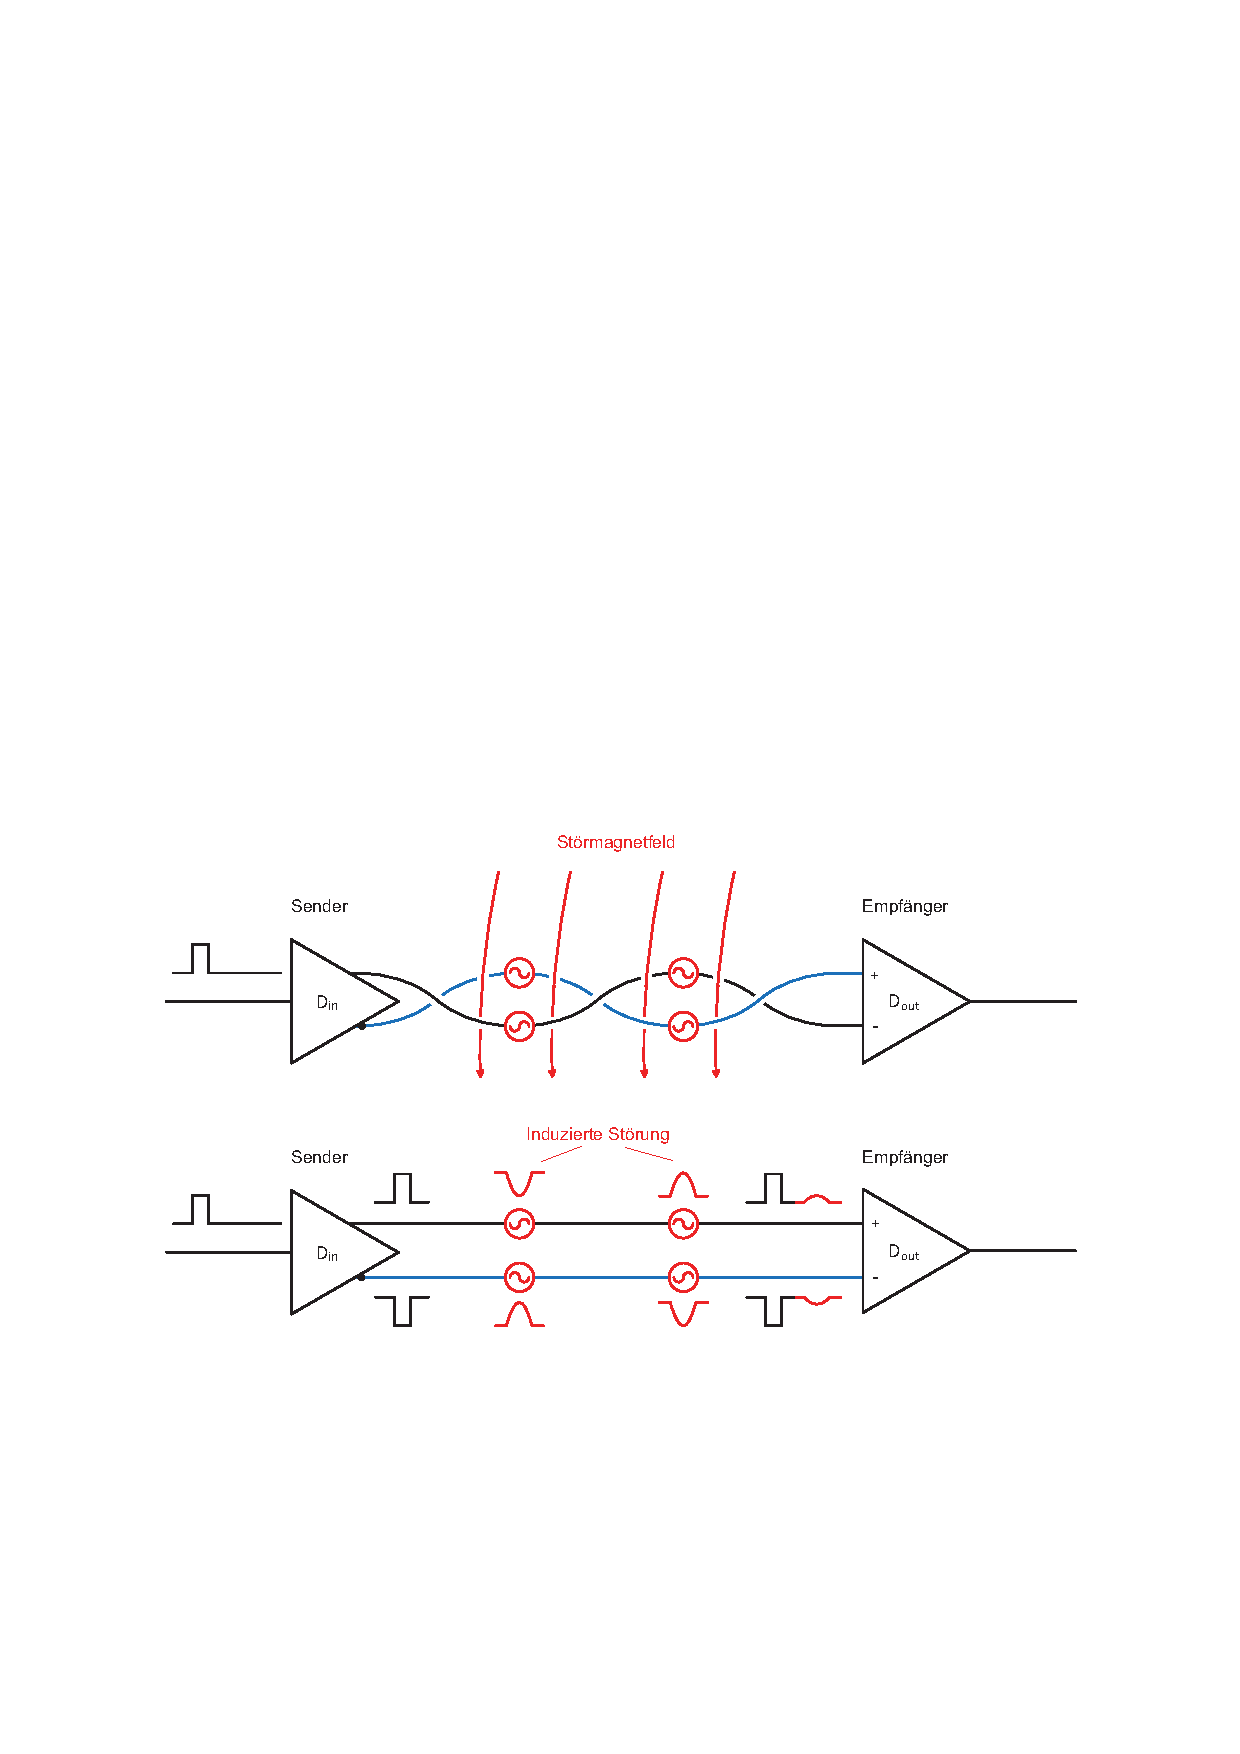
\includegraphics[width=0.8\textwidth]{images/differential.pdf}
	\caption{Differentielle Leitung \cite{{muellerkt1}}.}
	\label{fig.diff}
\end{figure}

Die Kollisions-Erkennung und -Auflösung wird über ID-Nummern der Teilnehmer gelöst. Vor dem Start einer Übertragung prüft der Teilnehmer, dass der Bus zur Zeit frei ist. Dann sendet der Teilnehmer seine ID-Nummer. Falls zwei Teilnehmer gleichzeitig zu senden beginnen, werden sie irgendwann unterschiedliche Bits senden. Der Teilnehmer, der dann das 'dominante' Bit sendet, liest vom Bus den gleichen Wert, den er gerade sendet. Für ihn ist die Übertragung nicht gestört. Der Teilnehmer mit dem 'rezessiven' Bit liest aber das 'dominante' Bit des anderen Senders und muss seine Übertragung sofort abbrechen. Diese Art der Kollisionsauflösung hat den Vorteil, dass keine Übertragungszeit verloren geht, da einer der Teilnehmer seine Nachricht senden darf. Der Verlierer wartet, bis der Bus wieder frei ist und probiert dann erneut, die Nachricht zu senden (vgl. \cite{boschcanspec2}).

Die korrekte Übertragung wird mittels eines \gls{crc}-Codes überprüft. Der Empfänger berechnet bereits während dem Empfang der Nachricht die \gls{crcgloss}-Prüfsumme. Sobald die vom Sender mitgeschickte CRC-Prüfsumme übertragen ist, kann der Empfänger diese mit der berechneten \gls{crc} vergleichen. Stimmen die Prüfsummen überein, bestätigt der Empfänger die korrekte Übertragung (vgl. \cite{boschcanspec2}).

\subsection{Speichermedium}
\paragraph{Kriterien} Das externe Speichermedium soll möglichst klein sein, wenig Stromverbrauch haben und einfach auswechselbar sein. Bei Inaktivität sollte das Medium wenn möglich keinen Strom verbrauchen. Für einen mehrwöchigen unabhängigen Betrieb einer Messstation muss genügend Speicherkapazität bereitgestellt werden.

\paragraph{Datenmenge} Pro \gls{sensor} werden bei hohem Geschiebeaufkommen maximal hundert \glspl{ereignis} pro Sekunde erwartet. Ein solches Geschiebeaufkommen stellt jedoch die Ausnahme dar. Ein \gls{ereignis} benötigt je nach verlangtem Detailgrad und Dauer des \gls{ereignis}ses 10--200 Byte Speicherplatz. Für den normalen Betriebsmodus werden 50 Byte/\gls{ereignis} gerechnet, bei 5 \glspl{ereignis}n pro Sekunde. Damit ergibt sich eine Datenrate von 250 Byte/s, die es pro \gls{sensor} abzuspeichern gilt. Mit zehn \glspl{sensor} im Einsatz müssen 2.5 kByte/s gespeichert werden. 

\paragraph{Unabhängige Betriebsdauer} Pro Gigabyte Speicherplatz können 111 Stunden Daten für zehn \glspl{sensor} gespeichert werden. Bei hohem Geschiebeaufkommen mit zwanzig mal mehr \glspl{ereignis}n bleiben immer noch 5 Stunden Aufzeichnungszeit pro Gigabyte. Begnügt man sich mit weniger Details, fallen pro \gls{sensor} in zehn Sekunden rund 400 Byte Daten an. Bei dieser Datenrate reicht ein Gigabyte für rund 700 Stunden. Auch bei hohem Geschiebeaufkommen kann die Anlage mehrere Tage an Daten speichern. 

\paragraph{Kapazität} Heute sind Speichermedien mit Kapazitäten bis über 128 GB erhältlich, so dass die Detailrate kein entscheidendes Kriterium mehr darstellt.

\paragraph{Datentransfer} Für den Transfer der Daten aus dem \gls{logger} auf einen Computer gibt es grundsätzlich zwei Varianten. Entweder man liest die Daten über eine Schnittstelle auf den Computer aus, oder man tauscht das Speichermedium aus. Das Auslesen via Schnittstelle benötigt zusätzlich Strom, das Wechseln des Speichermediums setzt einen mehr oder weniger komfortablen und trotzdem wasserdichten Zugang zum Medium voraus. Da heute Speichermedien mit kleinem Platzbedarf erhältlich sind, kann ein solcher Zugang recht einfach mit einem Schraubverschluss realisiert werden.

\paragraph{Vergleich} In Tabelle \ref{table.speichermedium} werden verschiedene Speichermedien miteinander verglichen. In der Spalte 'Breite' ist aufgelistet, wie gross eine Öffnung mindestens sein muss, um das Speichermedium wechseln zu können. 'Pins' gibt an, wie viele Leitungen für den Anschluss des Mediums am Microcontroller nötig sind. Der Stromverbrauch in Klammern ist für den Standby-Modus des Speichermediums.

\begin{table}
\begin{tabular}{|l|l|l|l|l|}
	\hline
	                      & \textbf{Breite} & \textbf{Pins} & \textbf{Stromverbrauch} & \textbf{Bemerkungen}        \\ \hline
	\textbf{SD-Card}      & 24 mm           & 9             & 20..100 mA (0.2 mA)     & 4 bit breiter serieller Bus \\ \hline
	\textbf{CompactFlash} & 43 mm           & 50            & max. 70 mA (k.A.)       & paralleler Bus              \\ \hline
	\textbf{USB-Stick}    & min. 12 mm      & 4             & typ. 70 mA (k.A.) &  \\ \hline
\end{tabular} 
\caption{Entscheidungsmatrix zur Auswahl des Speichermediums \cite{sdstd,cfstd,usbwiki}.}
\label{table.speichermedium}
\end{table} 

\paragraph{Entscheid} Für einen verschraubbaren Verschluss ist die CompactFlash-Karte zu breit, das Gehäuse würde dadurch sehr gross werden. Die SD-Karte und der USB-Stick sind vergleichbar in der Grösse. Von der SD-Karte sind auch kleinere Varianten erhältlich. Eine Öffnung für den Austausch des Speichermediums kann eine gewisse Grösse ohnehin nicht unterschreiten, damit hineingegriffen werden kann. Da die SD-Karte im Standby den geringeren Stromverbrauch hat, wird der \gls{logger} mit einem SD-Kartenleser ausgestattet.

\subsection{Sensor}
\todo{Sensorauswahl beschreiben}

\subsection{Schnittstelle}
Das gewählte \emph{NXP LPC4088 QuickStart Board} verfügt über einen \gls{usb}-Anschluss, über den eine serielle Schnittstelle angesprochen werden kann. Für eine einfache Kommandozeile oder ein Konfigurationsmenü ist diese Schnittstelle ausreichend. Die Schnittstelle kann mit einer Übertragunsrate von 9600 bis 115200 Baud betrieben werden. 


\subsection{Gehäuse}
Um den \gls{logger} und die \glspl{sensoreinh} wasserdicht zu verpacken, wurden Gehäuse und Komponenten mit der Schutzklasse IP68 gesucht. Die wasserdichten Gehäuse der Firma \emph{FIBOX} sind in verschiedenen Ausführungen erhältlich. Da diese Arbeit kein serienreifes Produkt zum Ziel hatte, wurden Gehäuse aus ABS-Kunststoff mit transparenten Deckeln gewählt. 

Die Stecker wurden ebenfalls mit Schutzklasse IP68 gewählt. Als zusätzliches Kriterium galt der Durchmesser des Kabelmantels. Die Stecker \emph{Lumberg 0332 05-1} verfügen über fünf Pole, die vierpolige Variante war zur Zeit nicht lieferbar.

Für den \gls{usb}-Anschluss gibt es wasserdichte Durchführungen, an denen sowohl innen als auch aussen Standard-USB-Kabel angeschlossen werden können. Die \emph{Buccaneer PCXP6043/B}-Gerätebuchse von \emph{Bulgin} erfüllt die Anforderungen. Für diese Buchse ist auch eine wasserdichte Kappe erhältlich.

Die verschraubbare Öffnung für die SD-Karte besteht aus einer M36/M32-Gewindebuchse, in die ein M32-Schraubdeckel eingeschraubt wird.


\section{Datenlogger}
Die Hardware-Architektur des \gls{logger}s ist in Abbildung \ref{fig.hw_logger} schematisch dargestellt. Kernstück ist der \gls{mc} \emph{NXP LPC4088}. Der \gls{mc} ist über eine serielle Schnittstelle mit dem CAN-Transceiver verbunden. Der Transceiver sendet Konfigurations- und Kontrolldaten und empfängt Messdaten über den CAN-Bus.

Dem \gls{mc} steht sowohl interner Programm- und Datenspeicher zur Verfügung, dieser ist aber sehr beschränkt. Damit Konfigurations- und Messdaten zwischengespeichert werden können, steht dem \gls{mc} auf dem \emph{NXP LPC4088 QuickStartBoard} (gestrichelter Kasten) mehr Speicher zur Verfügung: 8~MByte \gls{flash} und 32~MByte \gls{sdram}. Dieser Speicher genügt, um Daten von mehreren \glspl{sensoreinh} zwischenzuspeichern.

Über das \gls{mci} ist eine SD-Karte an den \gls{mc} angebunden. Auf der SD-Karte werden sowohl die Konfigurationsdaten als auch die Messdaten gespeichert. Heute sind SD-Karten mit bis zu 256~GByte Speicherplatz erhältlich (SDXC-Karten). Zur Zeit unterstützt die verwendete Bibliothek zur Verwendung der SD-Karten nur SDHC-Karten mit bis zu 32~GByte Speicherplatz. 

Für die Kommunikation mit einem \gls{compi} verfügt der \gls{logger} über einen \gls{usb}-Anschluss. Über einen \gls{terminalemu} wie \emph{PuTTY} kann via serielle Schnittstelle auf ein Konfigurationsmenü zugegriffen werden, um die Messanlage zu überwachen und zu steuern.

\begin{figure}
	\centering
		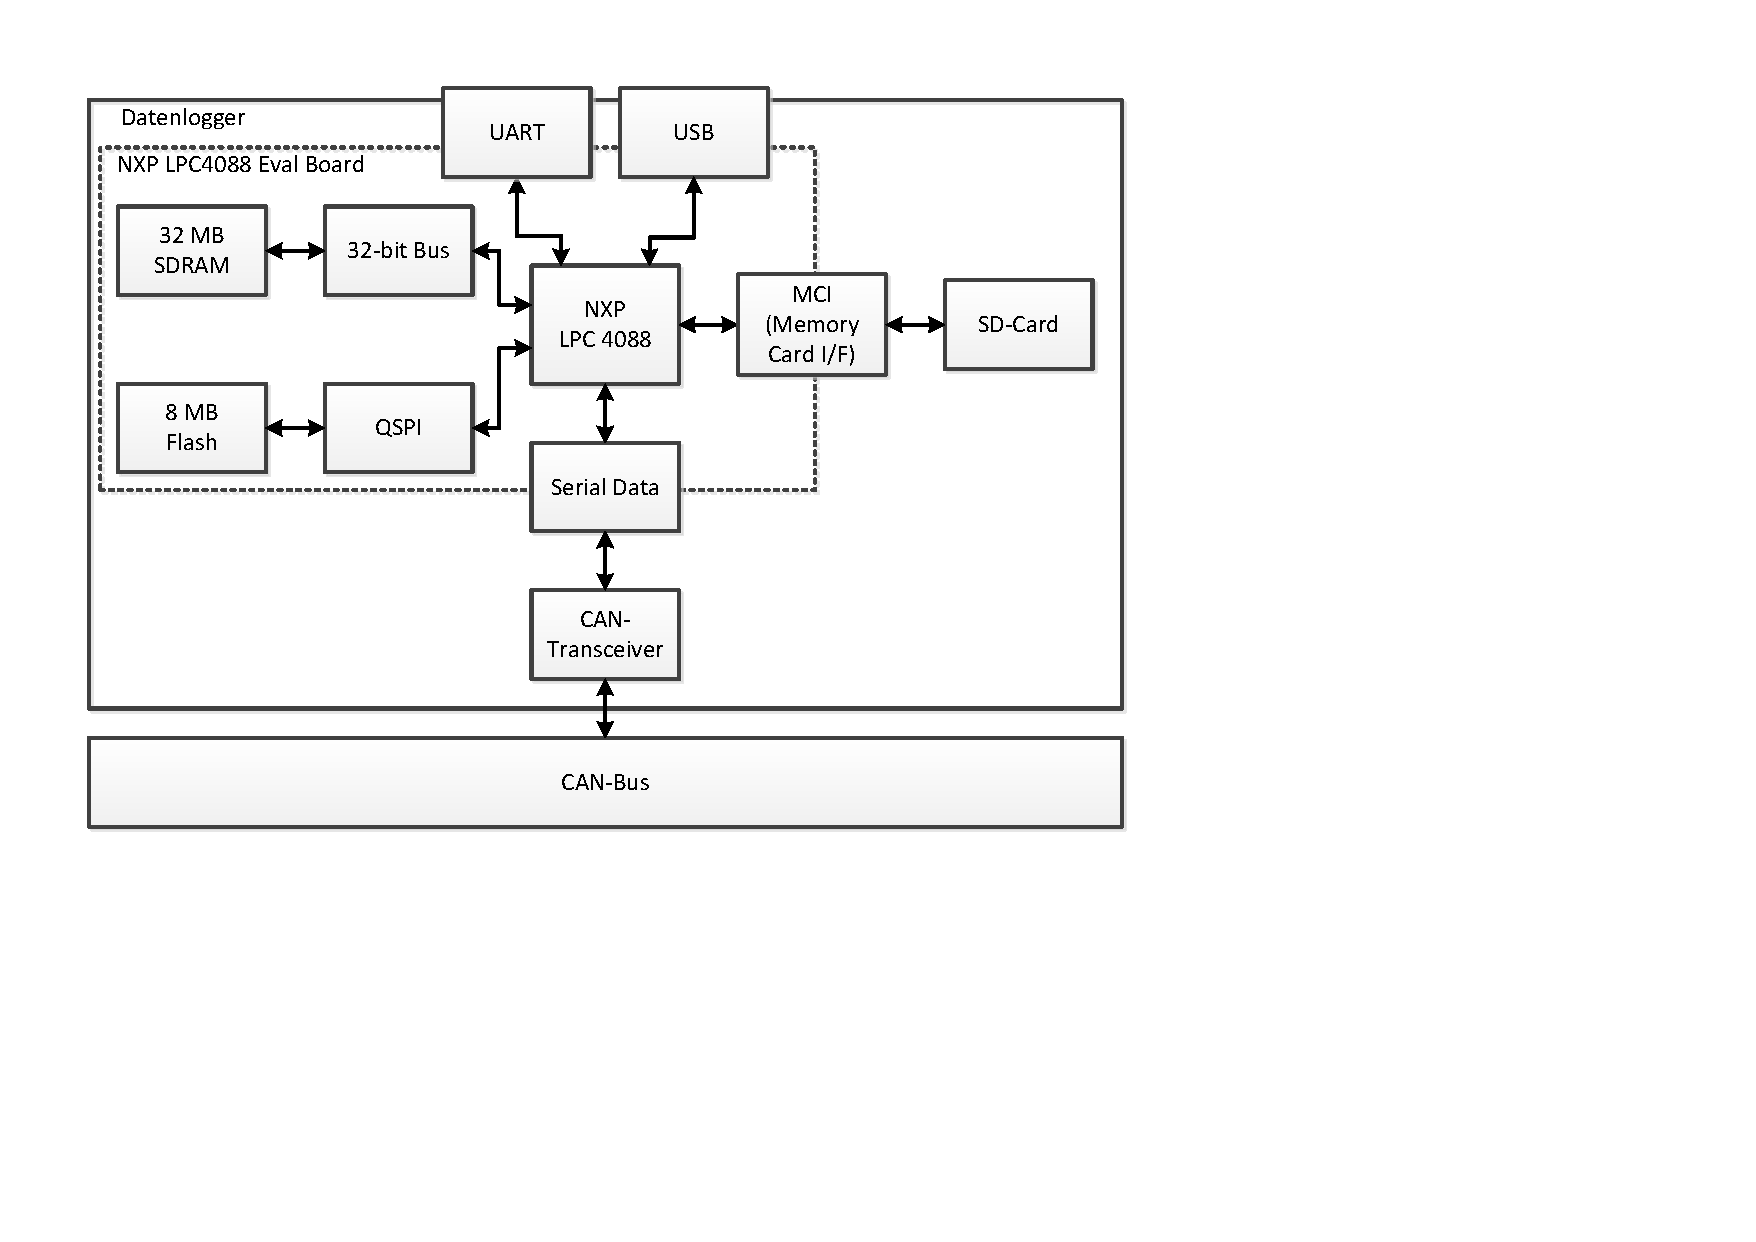
\includegraphics[width=0.8\textwidth]{images/visio/hardware_logger.pdf}
	\caption{Schematischer Hardware-Aufbau des \gls{logger}s.}
	\label{fig.hw_logger}
\end{figure}



\section{Sensoreinheit}
Die \gls{sensoreinh} ist ähnlich aufgebaut wie der \gls{logger}. Das Schema in Abbildung \ref{fig.hw_sensor} zeigt die Hardware. Wie der \gls{logger} ist der \emph{NXP LPC4088} \gls{mc} mit zusätzlichem \gls{sdram} und \gls{flash} ausgerüstet. Der Anschluss an den CAN-Bus ist identisch. Die SD-Karte wird in der \gls{sensoreinh} nicht benötigt und wurde deshalb weggelassen. Auch eine USB-Schnittstelle für die Konfiguration ist nicht nötig, da die Konfiguration über den CAN-Bus erfolgt.

Der Beschleunigungs-\gls{sensor} wird vom \emph{QuickStart Board} mit Spannung versorgt und gibt die gemessene Beschleunigung als analoge Spannung aus. Diese Spannung wird vom \gls{adwandler} des \emph{NXP LPC4088} \gls{mc} gemessen.

\begin{figure}
	\centering
		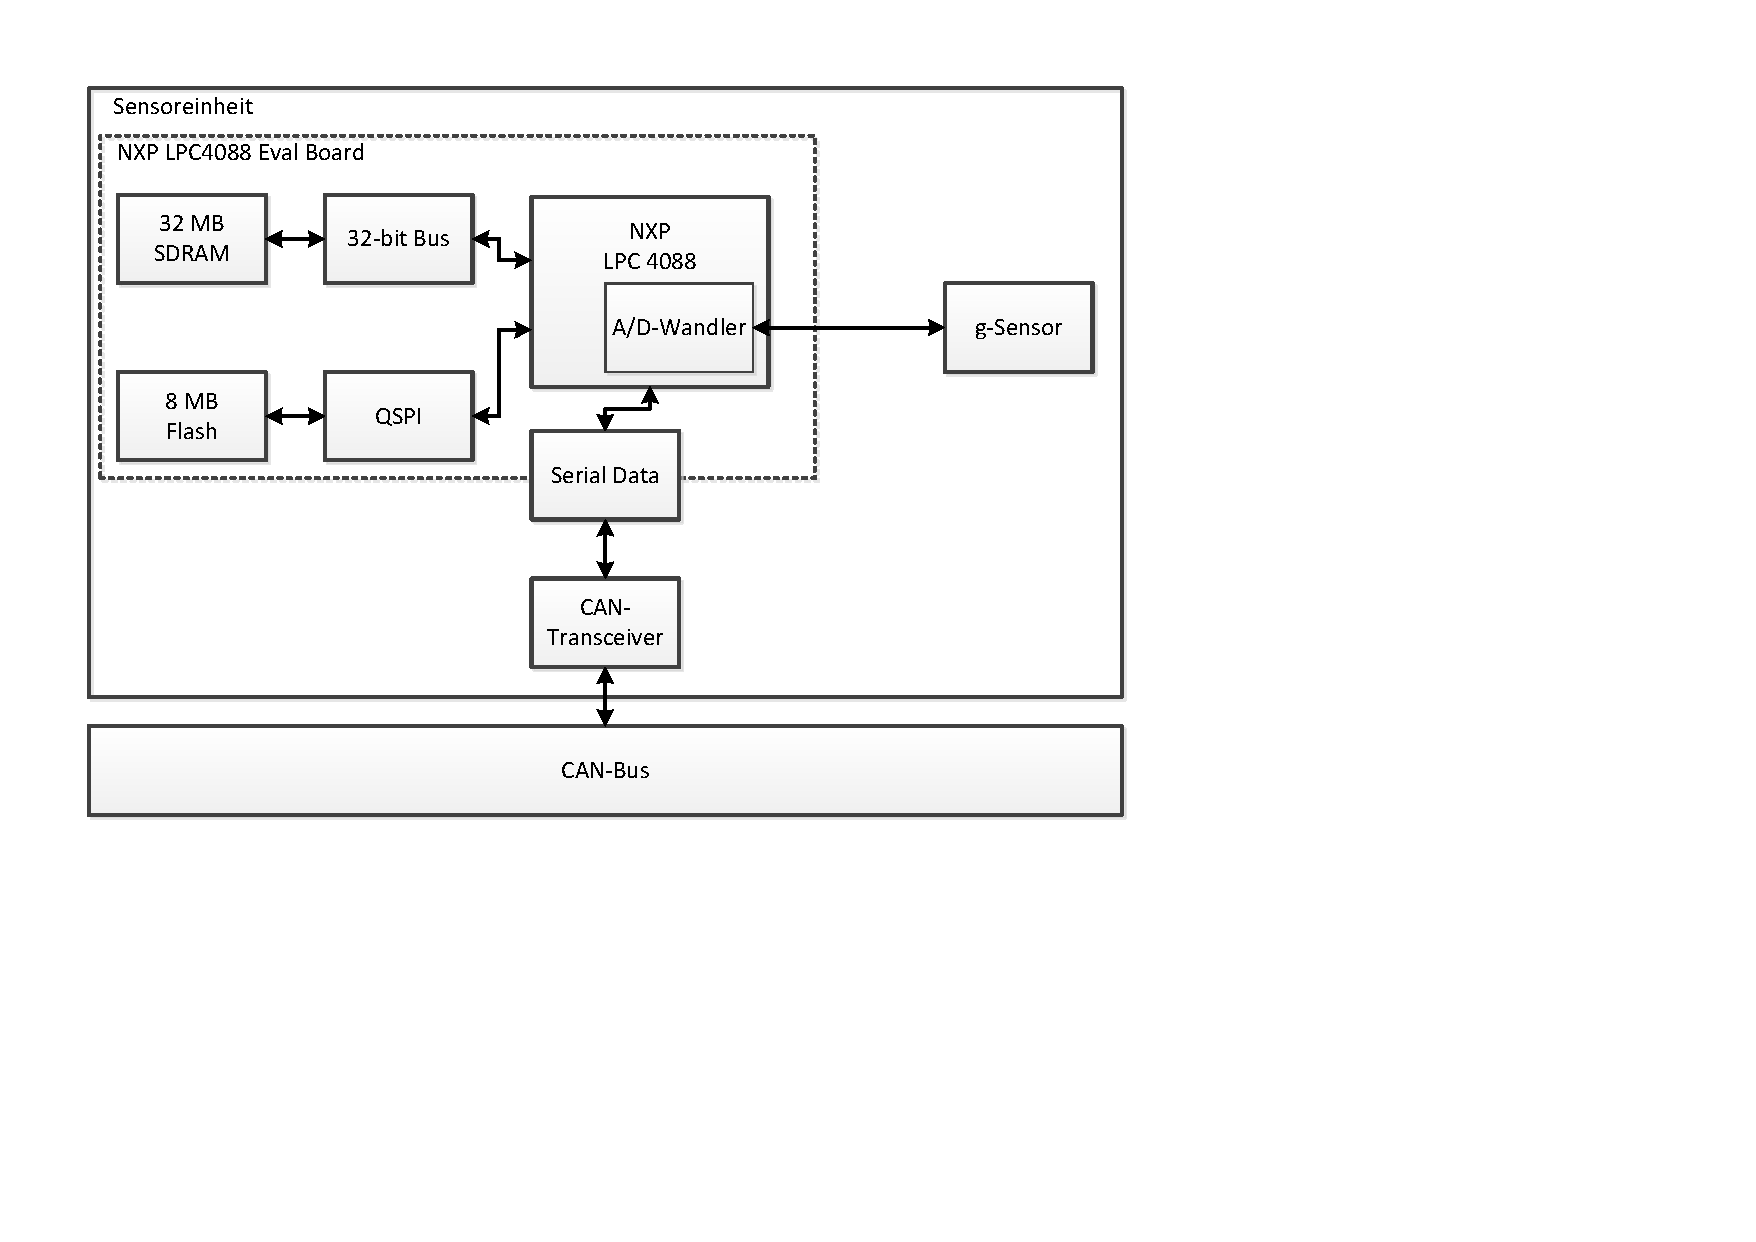
\includegraphics[width=0.8\textwidth]{images/visio/hardware_sensor.pdf}
	\caption{Schematischer Hardware-Aufbau der \gls{sensoreinh}.}
	\label{fig.hw_sensor}
\end{figure}


